\subsection{Contracts}
\subsubsection{Generic contracts}
\paragraph{Security contracts}
\subparagraph{Owned}
This contract is used to define the owner of a contract, in Soldino the owner is the address which 
do the deployment. The contract defines a modifier used to allow only the owner to call a function which uses the modifier.
\begin{figure}[H]
	\centering
	\frame{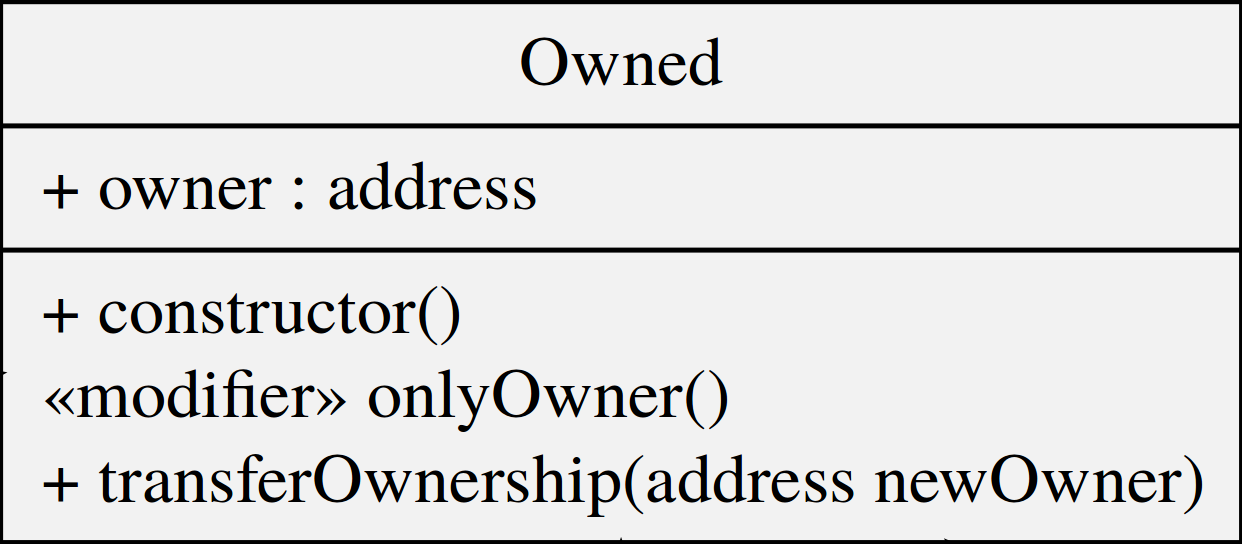
\includegraphics[scale=0.132]{res/images/solidity/owned.png}}
	\caption{class diagram of the Owned contract}
\end{figure}

\subparagraph{Authorizable}
This contract is used by all storage contracts. It's a derivate class of \texttt{Owned} and stores 
all the address which are authorized to call the functions that use the modifier \texttt{onlyAuthorized} defined in this contract.
\begin{figure}[H]
	\centering
	\frame{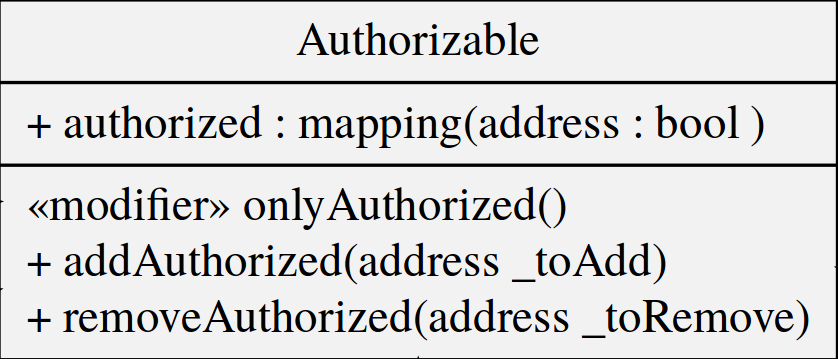
\includegraphics[scale=0.2]{res/images/solidity/authorizable.png}}
	\caption{class diagram of the Authorizable contract}
\end{figure}
\pagebreak
\paragraph{Token ERC20}\mbox{}\\

\noindent The contract \texttt{TokenCubit} implements the custom token \textit{Cubit}, this contract stores all the users' balance and defines all the methods in order to be ERC20 compliant.
\begin{figure}[H]
	\centering
	\frame{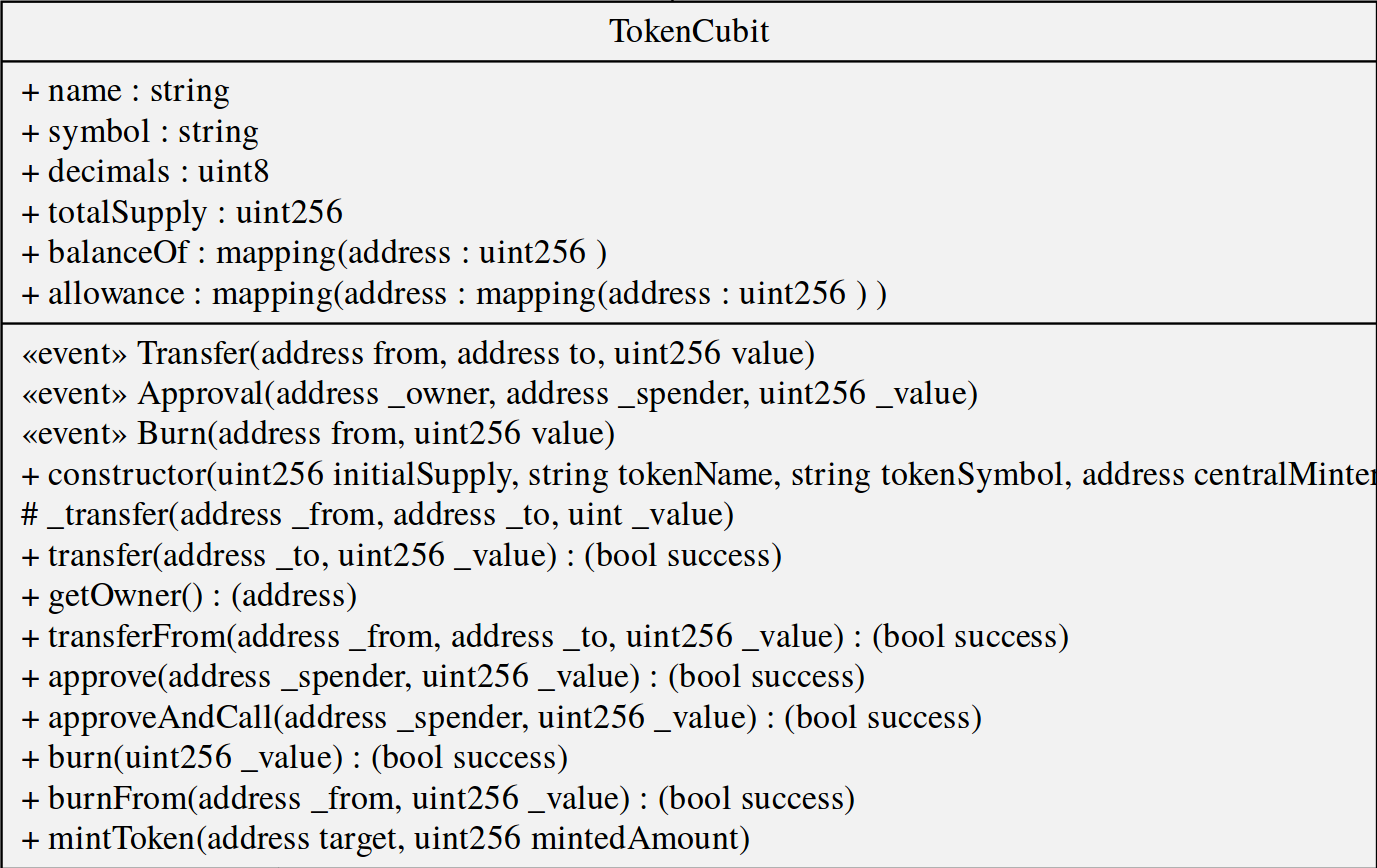
\includegraphics[scale=0.25]{res/images/solidity/tokencubit.png}}
	\caption{class diagram of the TokenCubit contract}
\end{figure}

\paragraph{ContractManager}\mbox{}\\ 

\noindent In order to achieve simple and cost effective upgradeability of the logic contracts \texttt{ContractManager} is used. This contract store a map in which the entries are composed in the following way:
\begin{itemize}
	\item\textbf{Key}: the contract name.
	\item\textbf{Value}: the last version of the contract deployment address.
\end{itemize}
When contract $A$ needs to communicate with another contract $B$, contract $A$ get the address of the last version of the contract $B$ from \texttt{ContractManager}. In this way there's no need to manage all references in the contracts. 
\begin{figure}[H]
	\centering
	\frame{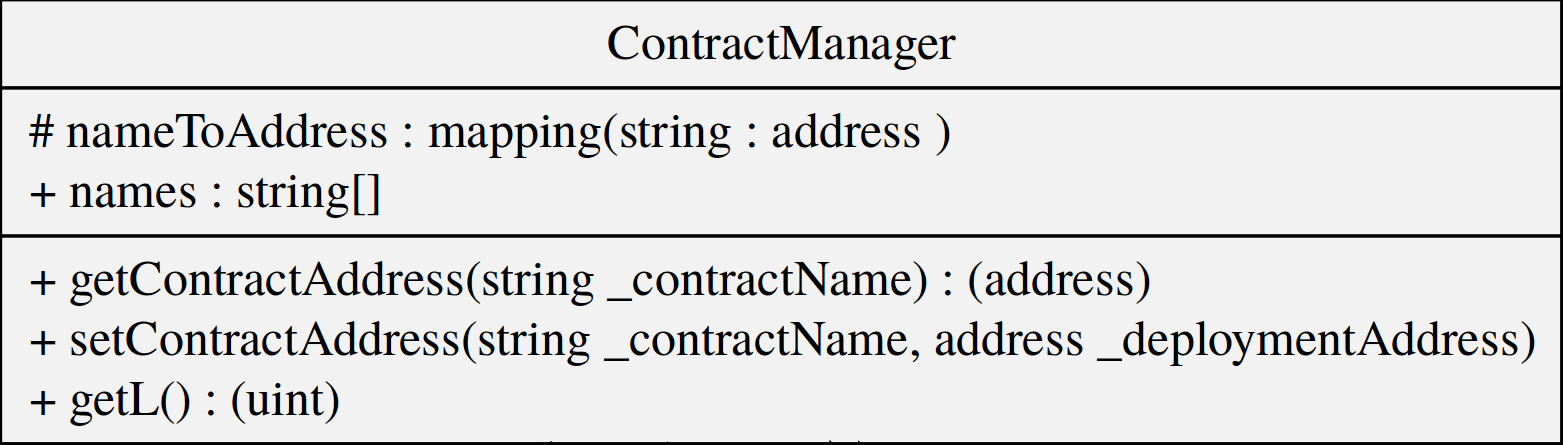
\includegraphics[scale=0.2]{res/images/solidity/contractmanager.png}}
	\caption{class diagram of the ContractManager contract}
\end{figure}
\pagebreak
\paragraph{Purchase}\mbox{}\\ 

\noindent The \texttt{Purchase} contract acts as a façade when it comes to buy products on Soldino.
Usually for every order (intended as one order for each seller) the user needs to confirm $n$ transaction, $n =$ number of orders, to buy all the products in his cart.\\
With the \texttt{Purchase} contract, the user has to confirm only two transaction independently how many products are in his cart. 
\begin{figure}[H]
	\centering
	\frame{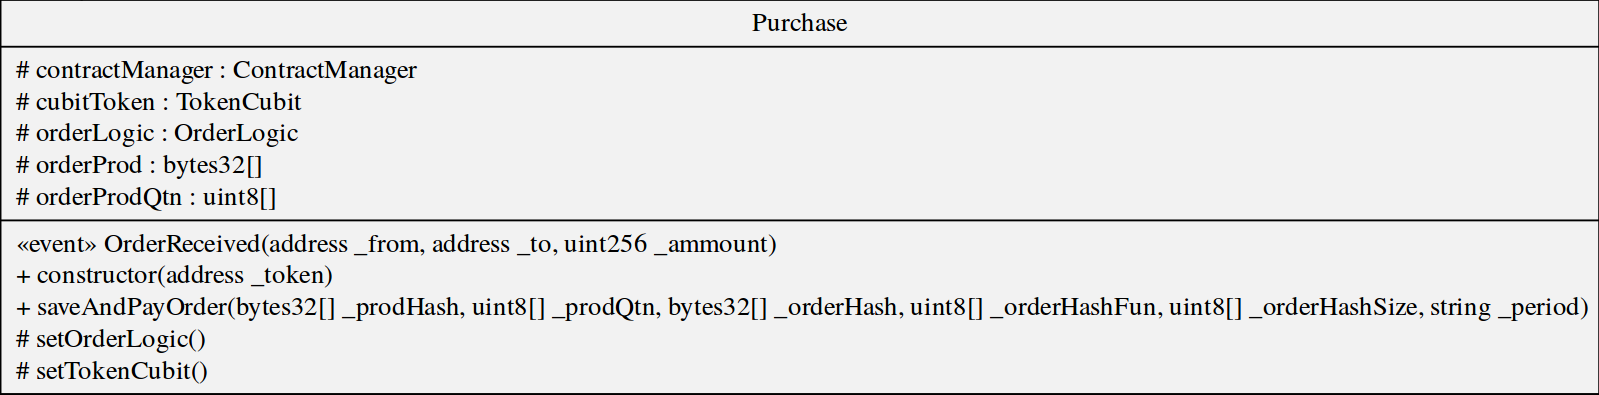
\includegraphics[scale=0.25]{res/images/solidity/purchase.png}}
	\caption{class diagram of the Purchase contract}
\end{figure}
\subsubsection{Storage contracts}
In this section we will illustrate the storage contracts. As mentioned before the storage contracts are immutable because they store all the critical data. In fact if a contract is upgraded, which means that a new version(using inheritance) is deployed, then all its state variable are new and the data of the previous version should be copied into the new contract, which translate in high cost transaction.\\
To avoid that, storage contracts implement no business logic of any kind. Their purpose is to store data and allow specific contract to modify their state. For data retrieval, on the other hand, the are no limitation because getter methods don't modify the storage contract's state.
All storage contracts inherit from \texttt{Authorizable} in order to use the \texttt{onlyAuthorized} modifier in the setter methods.
\paragraph*{Note: struct in the storage contract}

\paragraph{UserStorage}\mbox{}\\
This contract stores all the critical data of the users 
\begin{figure}[H]
	\centering
	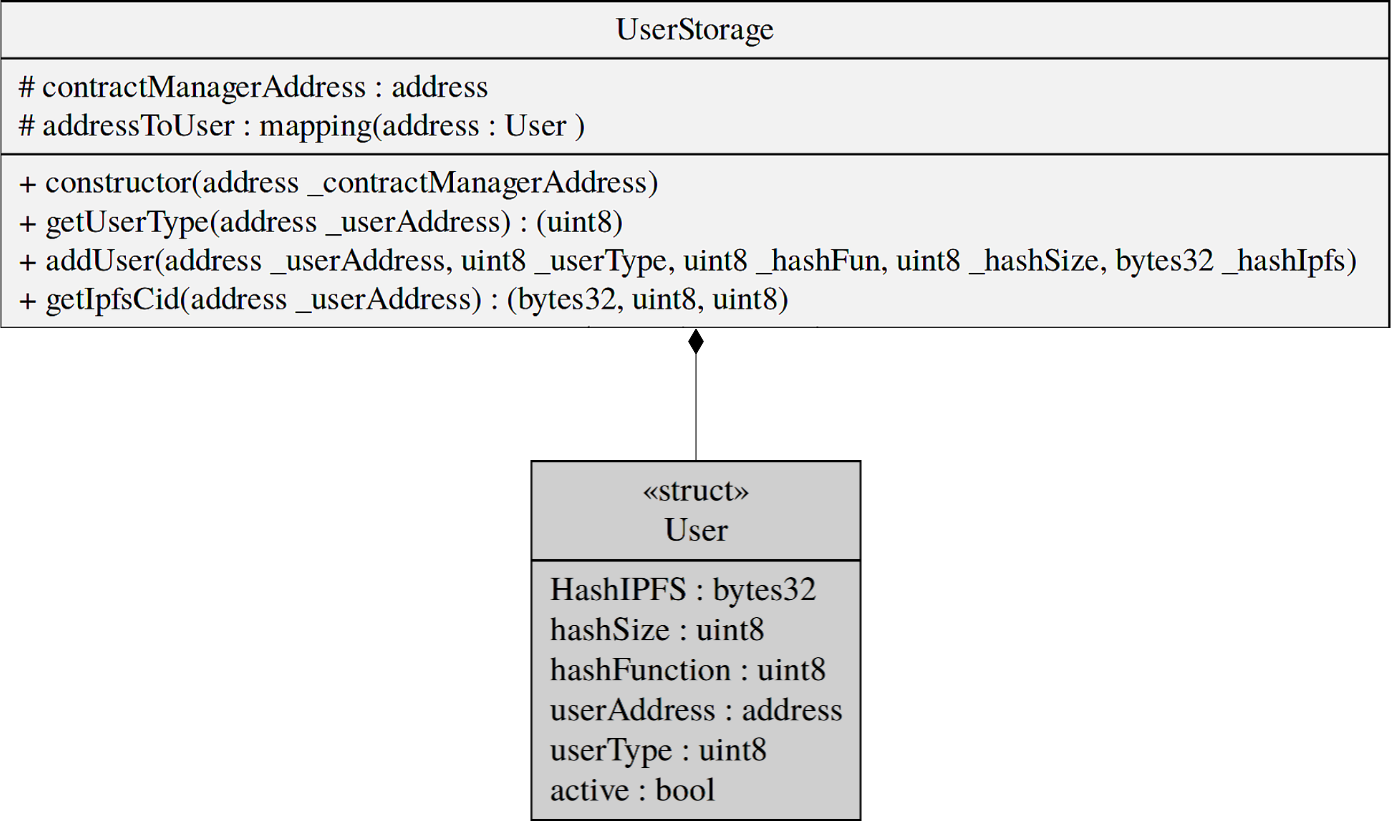
\includegraphics[scale=0.25]{res/images/solidity/userstorage.png}
	\caption{class diagram of the UserStorage contract}
\end{figure}
\pagebreak
\paragraph{ProductStorage}\mbox{}\\
\begin{figure}[H]
	\centering
	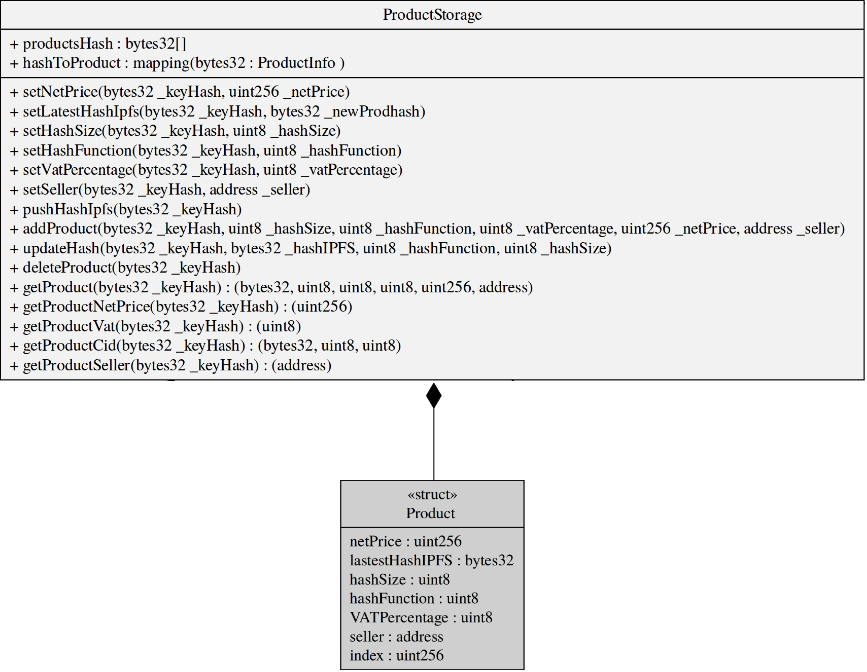
\includegraphics[scale=0.45]{res/images/solidity/productstorage.png}
	\caption{class diagram of the ProductStorage contract}
\end{figure}
\pagebreak
\paragraph{VatStorage}\mbox{}\\
\begin{figure}[H]
	\centering
	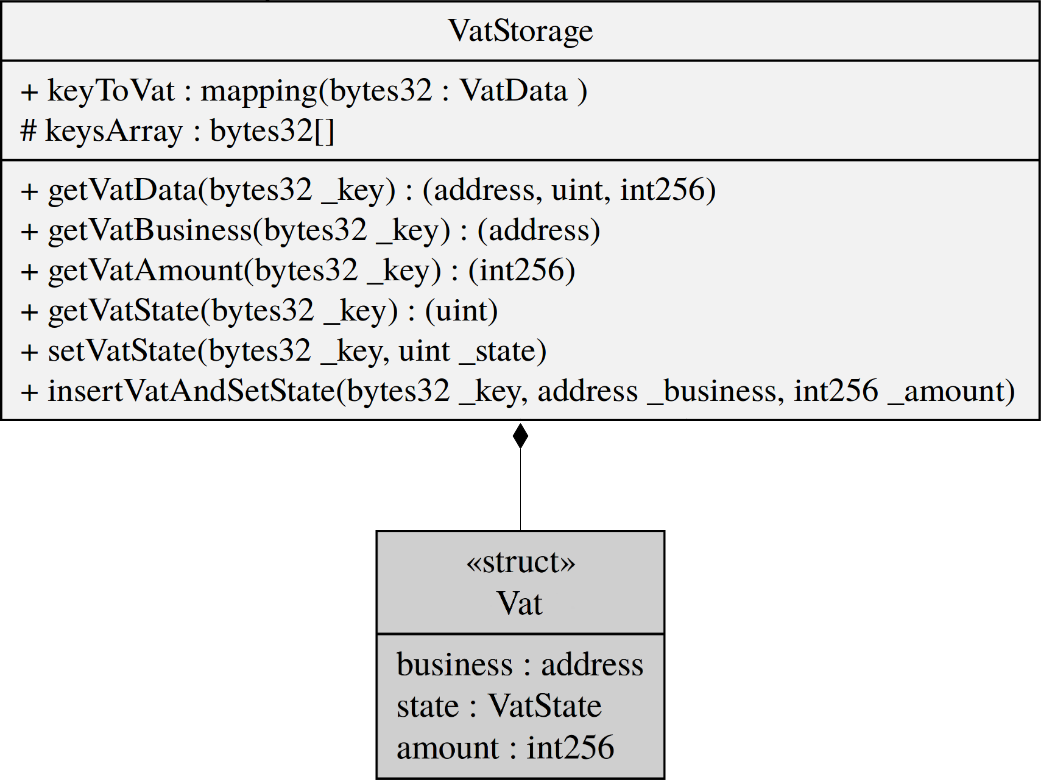
\includegraphics[scale=0.30]{res/images/solidity/vatstorage.png}
	\caption{class diagram of the VatStorage contract}
\end{figure}
\pagebreak
\paragraph{OrderStorage}\mbox{}\\
\begin{figure}[H]
	\centering
	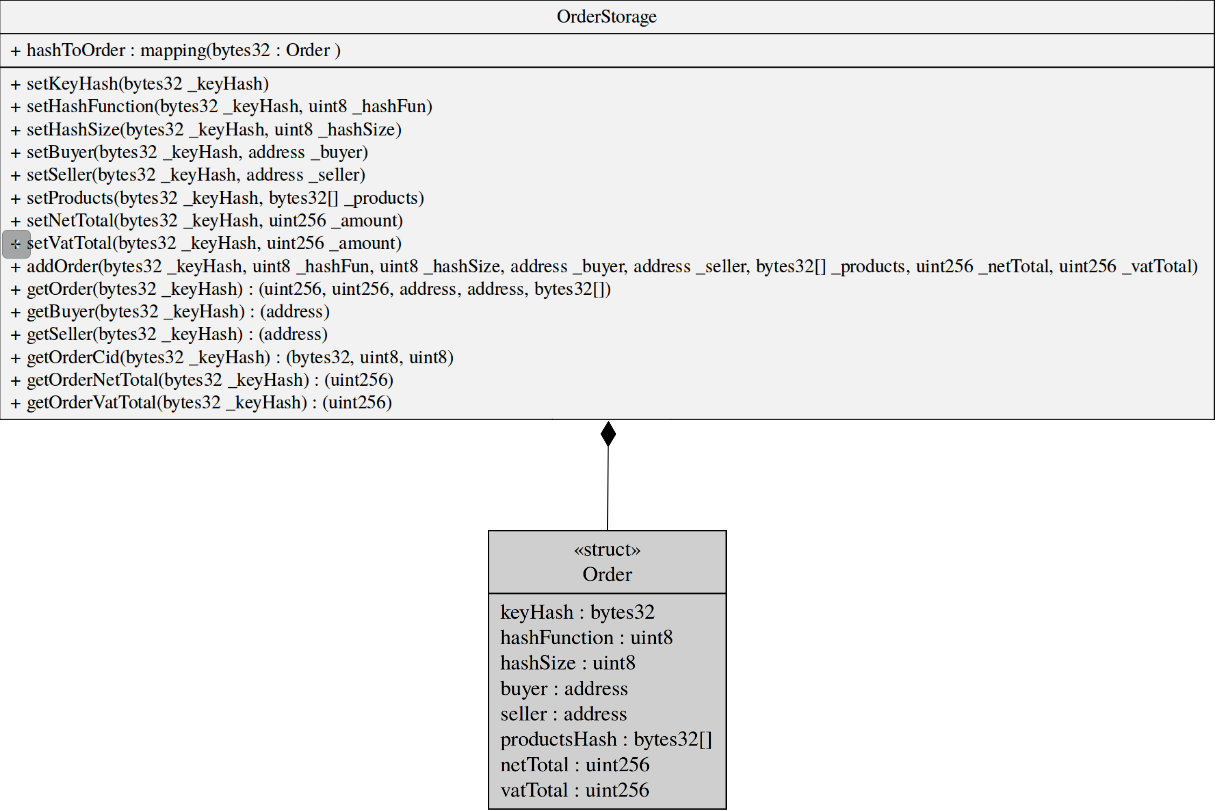
\includegraphics[scale=0.35]{res/images/solidity/orderstorage.png}
	\caption{class diagram of the OrderStorage contract}
\end{figure}

\subsubsection{Logic contracts}
\paragraph{UserLogic}\mbox{}\\
\begin{figure}[H]
	\centering
	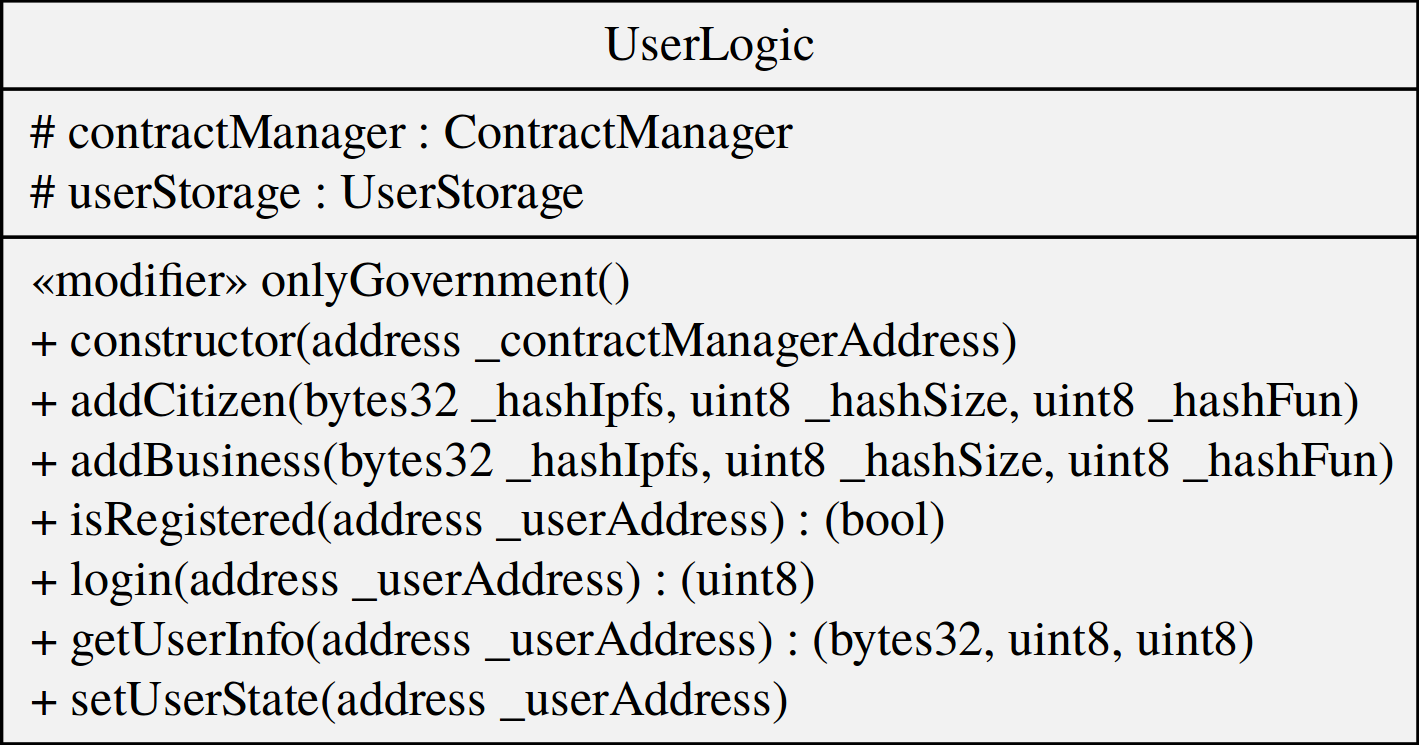
\includegraphics[scale=0.20]{res/images/solidity/userlogic.png}
	\caption{class diagram of the UserLogic contract}
\end{figure}

\paragraph{ProductLogic}\mbox{}\\
\begin{figure}[H]
	\centering
	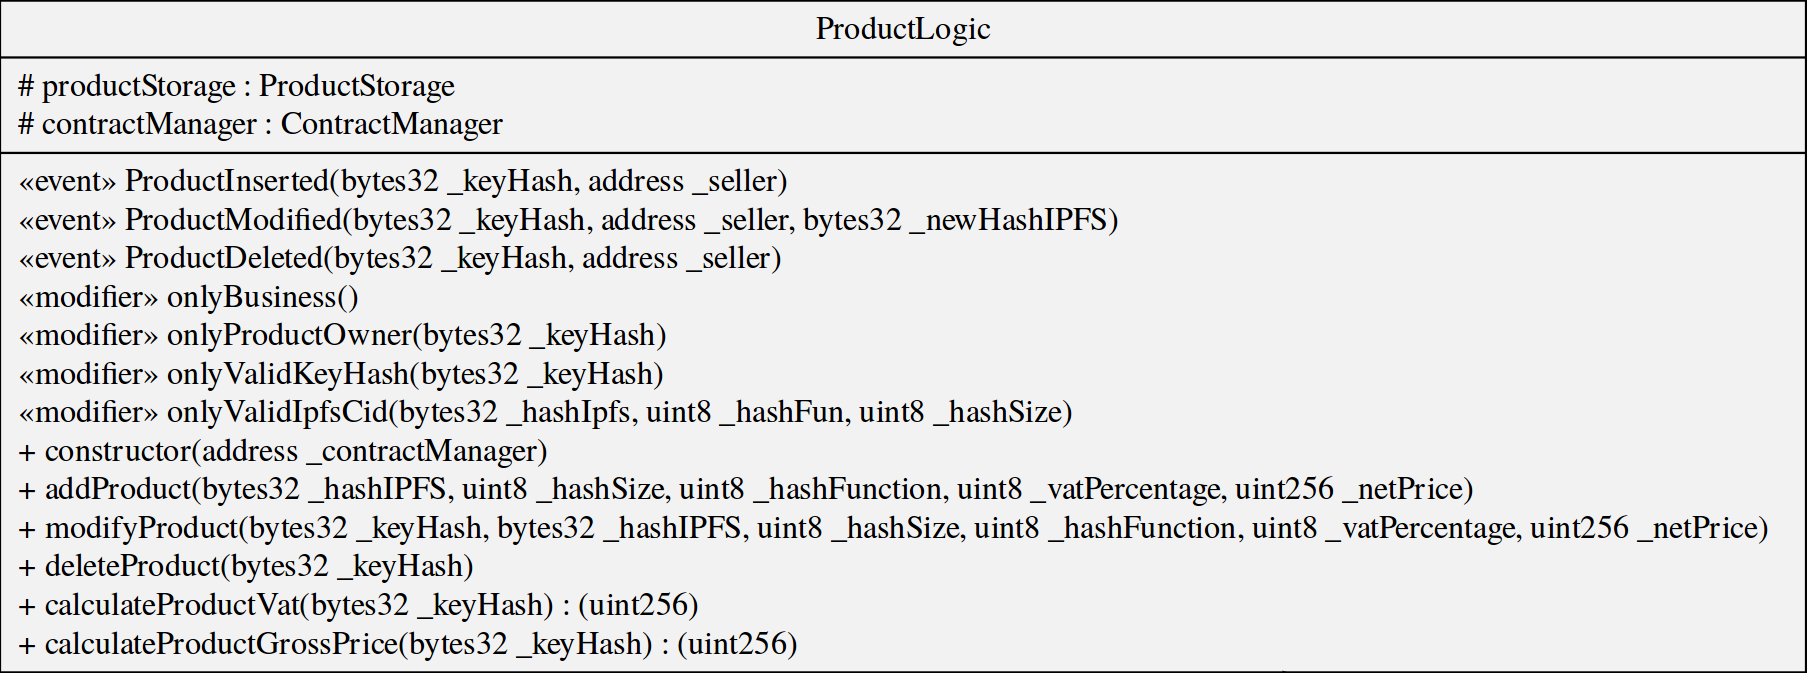
\includegraphics[scale=0.25]{res/images/solidity/productlogic.png}
	\caption{class diagram of the ProductLogic contract}
\end{figure}

\paragraph{VatLogic}\mbox{}\\
\begin{figure}[H]
	\centering
	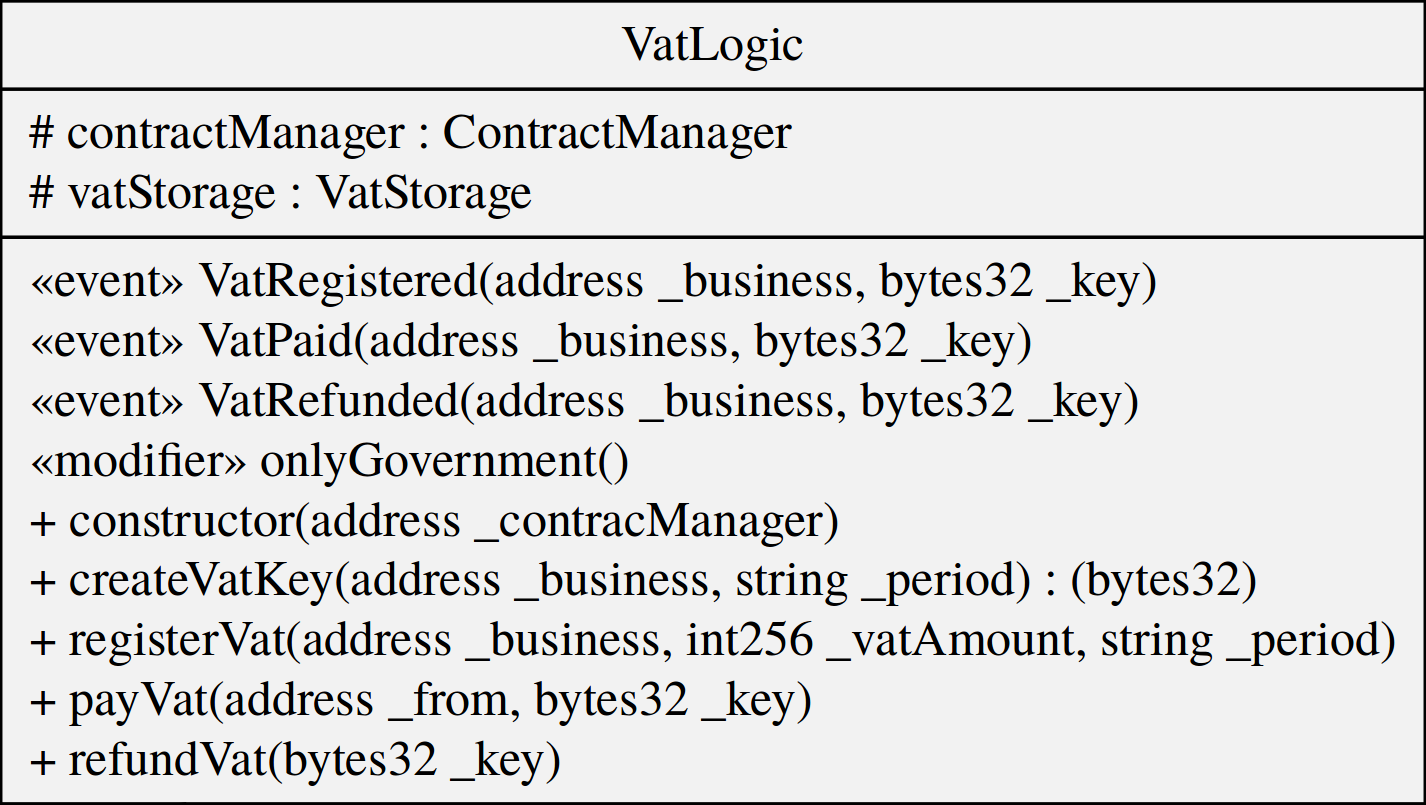
\includegraphics[scale=0.20]{res/images/solidity/vatlogic.png}
	\caption{class diagram of the VatLogic contract}
\end{figure}

\paragraph{OrderLogic}\mbox{}\\
\begin{figure}[H]
	\centering
	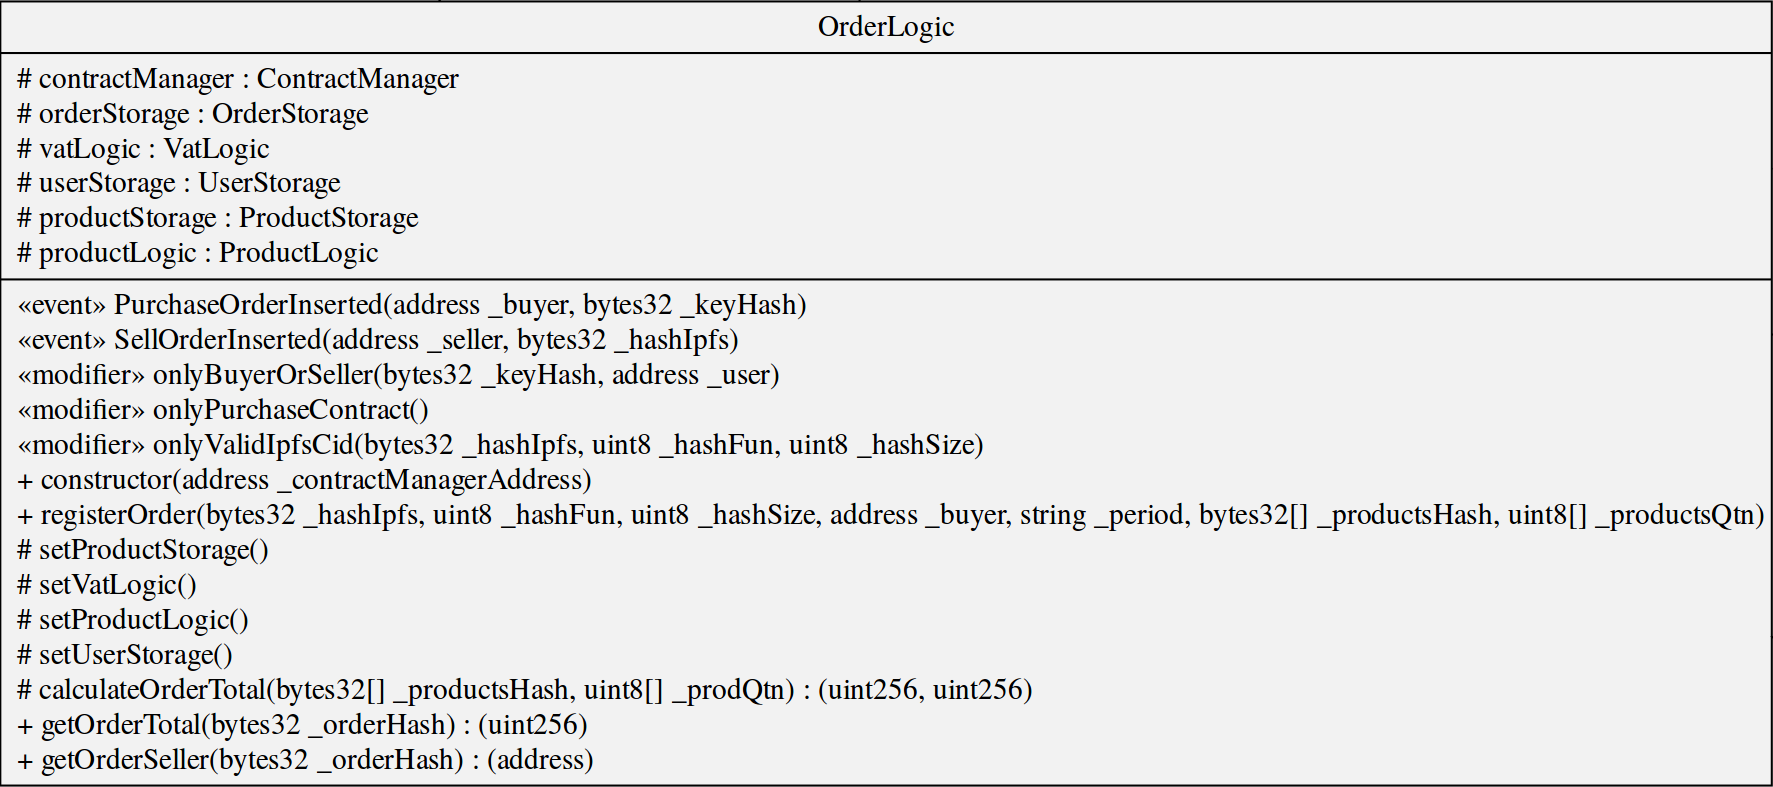
\includegraphics[scale=0.25]{res/images/solidity/orderlogic.png}
	\caption{class diagram of the OrderLogic contract}
\end{figure}